\documentclass[10pt,a4paper]{article}

\usepackage[a4paper,margin=17mm]{geometry}
\usepackage[T1]{fontenc}
\usepackage[utf8]{inputenc}
\usepackage{microtype}
\usepackage{amsmath,amssymb,bm}
\usepackage{array,booktabs,longtable,tabularx}
\usepackage{graphicx}
\usepackage{xcolor}
\usepackage{siunitx}
\usepackage{caption}
\usepackage{subcaption}
\usepackage{float}
\usepackage[hidelinks]{hyperref}
\usepackage{xurl}
\usepackage{enumitem}

\sisetup{per-mode=symbol, exponent-product=\cdot}
\setlength{\parindent}{0pt}
\setlength{\parskip}{0.45em}
\setlength{\tabcolsep}{3.5pt}
\renewcommand{\arraystretch}{1.12}
\setlist[itemize]{leftmargin=1.25em,itemsep=0.12em,topsep=0.2em}
\newcommand{\code}[1]{\texttt{\detokenize{#1}}}
\newcommand{\uu}{\bm u}
\newcommand{\xx}{\bm x}
\newcommand{\K}{\bm K}
\newcommand{\yy}{\bm y}
\newcommand{\thetas}{\bm\theta}
\newcommand{\GG}{\mathcal G}

\graphicspath{{figures/}}
\hypersetup{colorlinks=false}

\title{\textbf{DAMH--SMU inversion of the CD-A Niche 4 ERT20 support data}\\
\large Model parametrisation, likelihood construction, posterior diagnostics, and completion caveats}
\author{Generated from the local \code{inversion_atempt} campaign artifacts}
\date{Generated 2026-06-12 12:56; campaign \code{damh_ert20_smu_until_20260612_0830_v1}}

\begin{document}
\maketitle

\begin{abstract}
This paper-style report records the saved delayed-acceptance Metropolis--Hastings
surrogate-model-updating (DAMH--SMU) inversion for the two-year, 20-support
electrical-resistivity tomography (ERT20) observation operator around CD-A Niche 4.
The inversion samples a 207-dimensional physical/random-field parametrisation:
a tensor-valued intrinsic-permeability field, a porosity random field, and three
open-niche suction-curve controls.  The forward quantity learned by the surrogate is
the 20 by 35 support-averaged hydrologic response \(h_s(t;\thetas)\), transformed to
log10 resistivity by per-support bounded Archie fits inside the likelihood.  The
saved artifacts contain 2,083 exact OGS candidates, 2,057 accepted posterior trace
states, zero prerejections, and a best data-fit candidate
\code{solver01_eval000029} with local-Archie MAE 0.028417
log10.  The scientific result is usable as an empirical posterior diagnostic, but it
is not presented as a convergence-certified posterior or as a strict clean-finish
run: MPI shutdown stalled after file production stopped, the clean finish marker is
absent, and final combined MLP retraining did not run automatically.
\end{abstract}

\section*{Current Technical Position}

The ERT20 DAMH campaign should be read as a successful saved-candidate and
posterior-diagnostic run, not as a green strict-closeout run.  All indexed exact
candidate artifacts are complete and current for the 2,083 candidate directories;
the exact and combined datasets have the expected \(207\)-feature and \(700\)-observation
shapes; residual diagnostics pass with zero flagged issues.  The strict finish audit
fails only at the process/marker layer: output stopped before the morning handoff,
the process was no longer alive at audit time, but no \code{damh_finished} marker
was written after the MPI shutdown stall.  This distinction matters for reuse:
the exact OGS products are valid evidence, while the absent final combined MLP
checkpoint is a caveat.

\tableofcontents
\clearpage

\section{Model and Parametrisation}

The run keeps the OGS TRM model structure fixed and varies only a compact
inversion vector
\[
  \thetas =
  \left(k_0,\xi^K_1,\ldots,\xi^K_{100},\alpha,q,\phi_0,
  \xi^\phi_1,\ldots,\xi^\phi_{100},
  \Delta t_\mathrm{niche},s_\mathrm{niche},c_\mathrm{niche}\right)
  \in \mathbb R^{207} .
\]
The intrinsic-permeability tensor is written as a rotated, anisotropic random
field,
\[
  \K(\xx)=R(\alpha)
  \begin{bmatrix}
    10^{k_0 + f_K(\xx)} & 0\\
    0 & q\,10^{k_0 + f_K(\xx)}
  \end{bmatrix}
  R(\alpha)^T,
\]
where \(f_K\) is the 100-mode permeability random field.  Porosity is represented
by a homogeneous level plus a 100-mode bounded/logit random-field perturbation.
The three open-niche controls shift, scale, and offset the prescribed suction
history; this is deliberately lower-dimensional than releasing an arbitrary
boundary curve.

\begin{table}[H]
\centering
\scriptsize
\begin{tabular}{p{0.20\linewidth}p{0.34\linewidth}p{0.36\linewidth}}
\toprule
Parameter & Prior / treatment & Role \\
\midrule
$k_0$ & $\mathcal{N}(-21.02,5.1^2)$ & global log10 intrinsic-permeability level \\
$\alpha$ & $\mathcal{N}(139.9,5^2)$ & bedding-aligned tensor rotation \\
$q=K_{22}/K_{11}$ & $\mathcal{U}(0.1,0.9)$ & local anisotropy ratio before rotation \\
$\phi_0$ & trunc. $\mathcal{N}(0.1504,0.012^2)$ on [0.05, 0.175] & mean porosity level before RF perturbation \\
$\Delta t_{\rm niche}$ & trunc. $\mathcal{N}(92.09,35^2)$ on [0, 260] & open-niche suction-curve time shift \\
$s_{\rm niche}$ & trunc. $\mathcal{N}(1.23,0.15^2)$ on [0.65, 1.35] & open-niche suction-curve amplitude multiplier \\
$c_{\rm niche}$ & trunc. $\mathcal{N}(0.2434,0.6^2)$ on [-2, 2] & open-niche suction offset \\
$\xi^K_1,\ldots,\xi^K_{100}$ & independent normal prior entries & permeability KL coefficients on the mesh \\
$\xi^\phi_1,\ldots,\xi^\phi_{100}$ & independent normal prior entries & porosity random-field coefficients \\
$a_s,b_s$ & bounded least-squares, not sampled & per-support Archie intercept and slope fitted inside likelihood \\
\bottomrule
\end{tabular}

\caption{Active parametrisation and prior/treatment summary.  The Archie
parameters \(a_s,b_s\) are not DAMH state variables in this campaign; they are
refitted by bounded least squares for every exact candidate and every support.}
\label{tab:priors}
\end{table}

\begin{figure}[H]
\centering
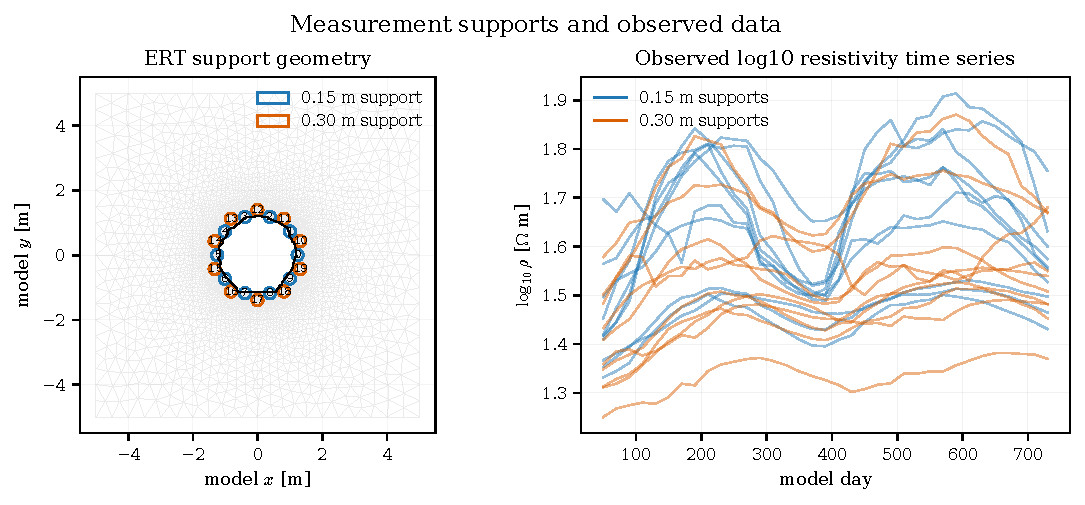
\includegraphics[width=0.98\linewidth]{fig01_supports_and_measurements.pdf}
\caption{ERT support design and observed data used by the inversion.  Supports
0--9 lie approximately \(0.15\,\mathrm{m}\) from the niche boundary; supports
10--19 lie approximately \(0.30\,\mathrm{m}\) from the boundary and are angularly
interlaced with the inner ring.}
\label{fig:supports}
\end{figure}

\section{Observation Operator and Likelihood}

For each candidate state \(\thetas\), OGS provides a support/time hydrologic
response \(h_s(t;\thetas)\), stored as a \(20\times35\) array.  The ERT prediction
uses a local Archie form per support,
\[
  \GG_{s,t}(\thetas,a_s,b_s) = a_s + b_s h_s(t;\thetas),
\]
with \(a_s\in[-0.7,1.3]\) and \(b_s\in[-2.0,-0.2]\).  These two parameters are
fitted independently for each support by bounded least squares before the
likelihood is evaluated.  The measurement noise model is Gaussian in log10
resistivity with support-series standard deviation
\[
  \sigma_\rho = 0.18.
\]
The likelihood uses an effective independent row count of
\(80\)
over the 700 support/time observations, so the dense time series is intentionally
down-weighted relative to its raw row count.

\[
 \log L(\thetas) =
 \sum_i w_i\left[
 -\frac12\left(\frac{\GG_i(\thetas)-y_i}{\sigma_\rho}\right)^2
 -\frac12\log(2\pi\sigma_\rho^2)
 \right].
\]

\begin{figure}[H]
\centering
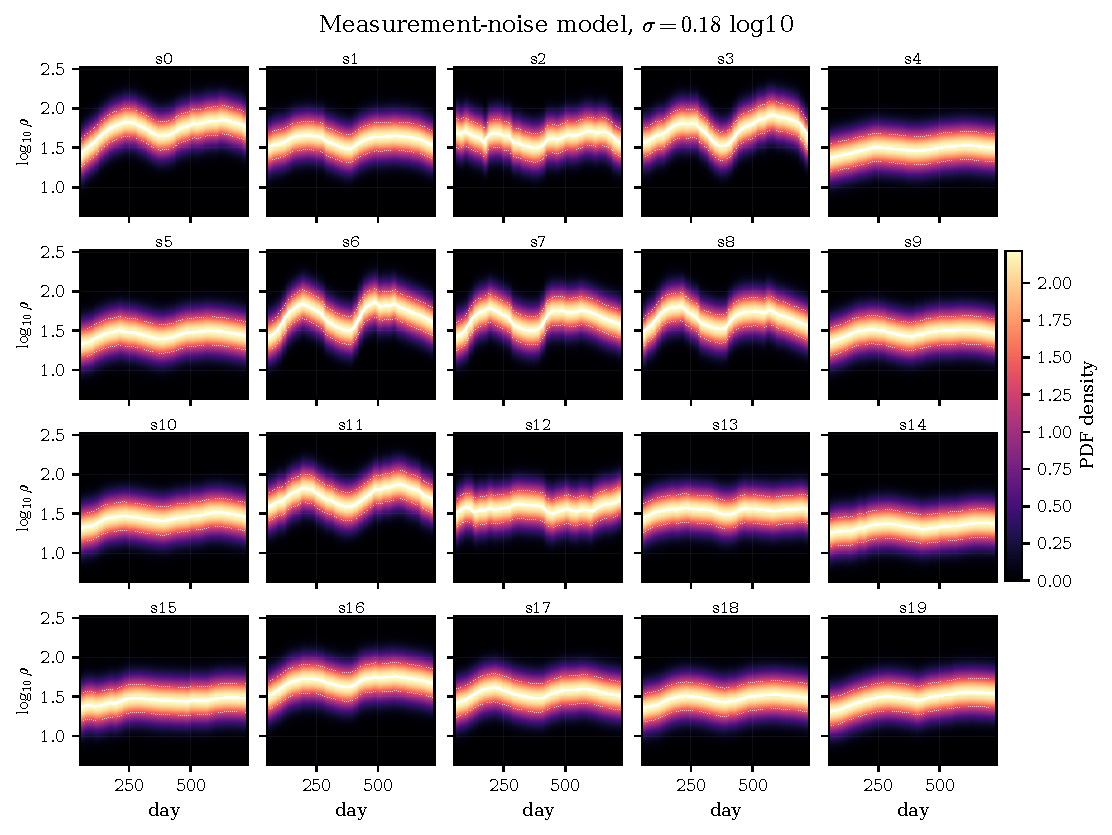
\includegraphics[width=0.98\linewidth]{fig02_measurement_noise_pdf_20_supports.pdf}
\caption{The measurement-noise density actually used by the likelihood, drawn
around the observed support time series.  This figure is separate from posterior
predictive uncertainty: it is the assumed data error model.}
\label{fig:noise}
\end{figure}

\section{DAMH--SMU Run}

The DAMH--SMU run used the neural surrogate to propose and screen states, while
the saved exact candidate set stores the corresponding OGS evaluations and local
Archie refits.  The exact candidate directories, candidate index, Archie
observation manifest, parameter trace, and residual diagnostics are mutually
current.  The trace has very high acceptance in this late local region of
parameter space; therefore the accepted states are useful for local uncertainty
diagnostics, but they should not be over-sold as an independent posterior sample.

\begin{table}[H]
\centering
\small
\begin{tabularx}{\linewidth}{@{}p{0.43\linewidth}X@{}}
\toprule
Quantity & Value \\
\midrule
Campaign & \code{damh\_ert20\_smu\_until\_20260612\_0830\_v1} \\
Exact OGS candidates & 2e+03 \\
Accepted / rejected / prerejected trace rows & 2057 / 11 / 0 \\
Trace acceptance ratio & 0.99468 \\
Exact dataset shape & $X=(2083,207)$, $h=(2083,700)$ \\
Combined dataset shape & $X=(4063,207)$, $h=(4063,700)$ \\
Support/time observations & $20\times35=700$ \\
Candidate production rate & 187.6 exact candidates h$^{-1}$ \\
Best data-fit candidate & \code{solver01\_eval000029} \\
Best local Archie log-likelihood & 61.7063 \\
Best local Archie MAE & 0.028417 log10 \\
Strict finish marker & absent \\
Process alive at audit & no \\
\bottomrule
\end{tabularx}

\caption{Campaign summary from the saved manifests and generated audits.}
\label{tab:campaign}
\end{table}

\begin{figure}[H]
\centering
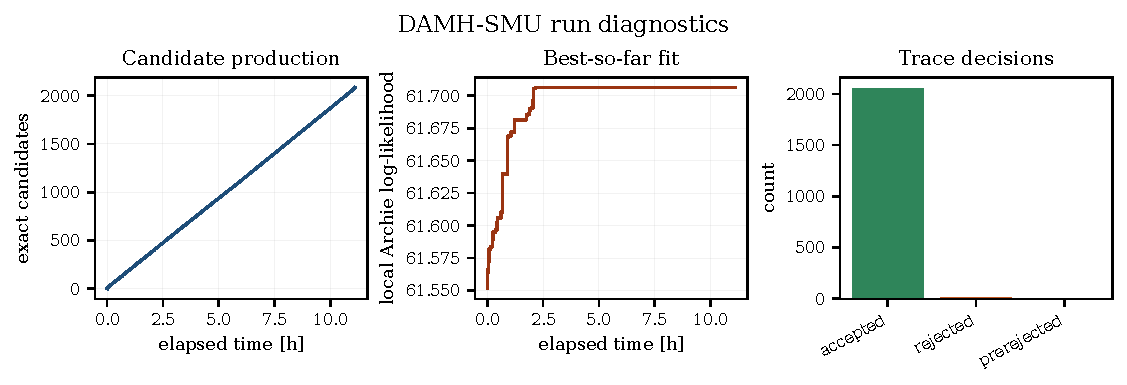
\includegraphics[width=0.98\linewidth]{fig03_run_diagnostics.pdf}
\caption{Run diagnostics.  Candidate production was steady until the morning
window; the best local-Archie likelihood plateaued in a narrow region; the trace
contains 2,057 accepted and 11 rejected decisions, with no prerejections.}
\label{fig:run}
\end{figure}

\begin{table}[H]
\centering
\small
\begin{tabularx}{\linewidth}{@{}p{0.55\linewidth}X@{}}
\toprule
Quantity & Value \\
\midrule
Sampler ranks & 2e+01 \\
Trace rows per rank, min / median / max & 129 / 1e+02 / 146 \\
$k_0$ median IACT & 47.5 \\
$\phi_0$ median IACT & 37.4 \\
$\Delta t_{\rm niche}$ median IACT & 33.9 \\
$s_{\rm niche}$ median IACT & 28.9 \\
\bottomrule
\end{tabularx}

\caption{Chain length and simple integrated-autocorrelation-time diagnostics.
The short rank-local chains and high acceptance motivate the report language:
empirical posterior diagnostics, not a convergence-certified posterior.}
\label{tab:chain}
\end{table}

\section{Best Fit and Residual Structure}

The top candidates are all close neighbours from rank 1, with almost identical
Archie objectives and hydrologic parameters.  The best data-fit candidate is
\code{solver01_eval000029}, with local-Archie objective
0.049063, MAE 0.028417
log10, \(k_0=-21.062\), \(\phi_0=0.14689\),
and niche-curve shift 96.082 days.

\begin{table}[H]
\centering
\scriptsize
\begin{tabular}{rp{0.25\linewidth}rrrrr}
\toprule
Rank & Candidate & $\ell$ & MAE & $k_0$ & $\phi_0$ & $\Delta t$ \\
\midrule
1 & \code{solver01\_eval000029} & 61.7063 & 0.028417 & -21.062 & 0.14689 & 96.082 \\
2 & \code{solver01\_eval000028} & 61.7054 & 0.028444 & -21.045 & 0.14678 & 96.969 \\
3 & \code{solver01\_eval000030} & 61.703 & 0.028488 & -21.087 & 0.14701 & 95.723 \\
4 & \code{solver01\_eval000027} & 61.6906 & 0.028546 & -21.022 & 0.14725 & 96.879 \\
5 & \code{solver01\_eval000026} & 61.6899 & 0.028564 & -21.045 & 0.14747 & 97.035 \\
6 & \code{solver01\_eval000025} & 61.686 & 0.028607 & -21.046 & 0.14752 & 96.46 \\
7 & \code{solver01\_eval000024} & 61.6853 & 0.0286 & -21.056 & 0.14697 & 96.873 \\
8 & \code{solver01\_eval000017} & 61.6813 & 0.028632 & -21.038 & 0.14801 & 96.025 \\
\bottomrule
\end{tabular}

\caption{Top exact OGS candidates ranked by local-Archie log likelihood.}
\label{tab:top-candidates}
\end{table}

\begin{figure}[H]
\centering
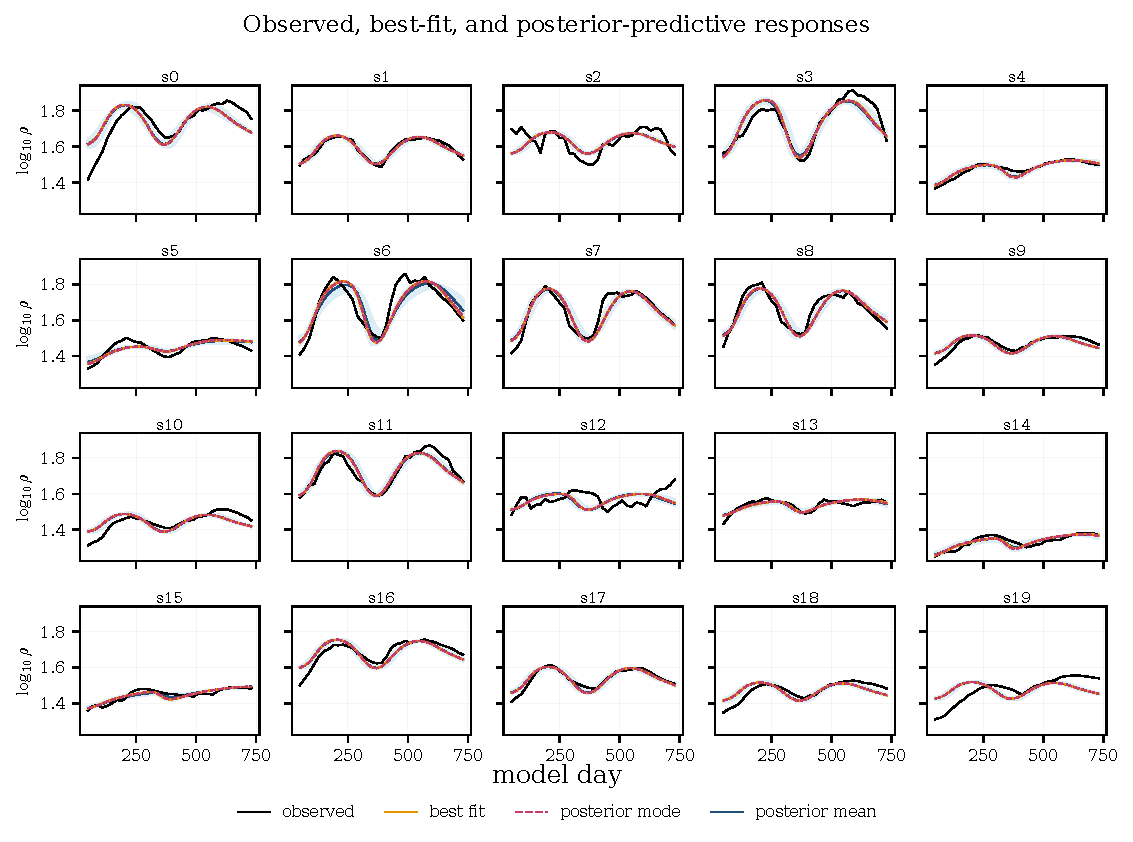
\includegraphics[width=0.98\linewidth]{fig04_best_fit_posterior_20_supports.pdf}
\caption{Observed log10 resistivity, best-fit prediction, posterior-mode
prediction, posterior mean, and the empirical 90\% posterior-predictive band for
each ERT support.}
\label{fig:bestfit20}
\end{figure}

\begin{figure}[H]
\centering
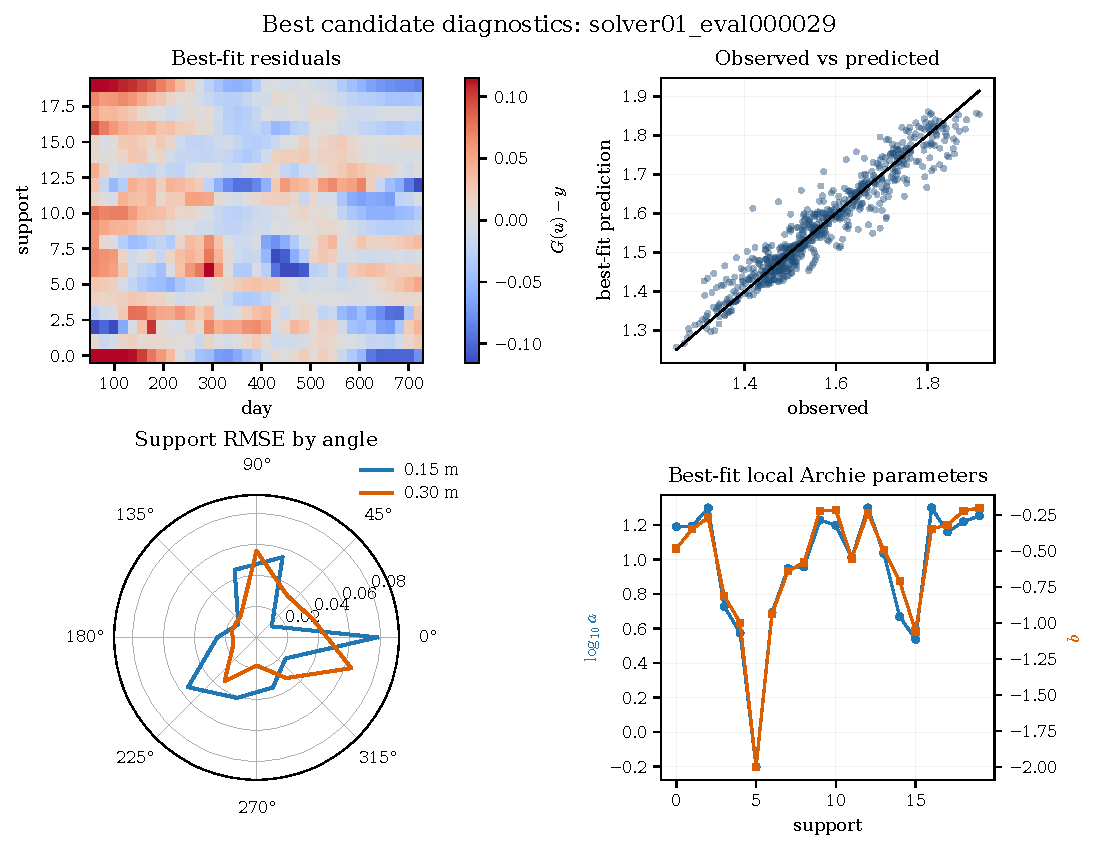
\includegraphics[width=0.98\linewidth]{fig05_best_fit_residual_archie.pdf}
\caption{Best-candidate residual structure and per-support Archie coefficients.
The polar panel has exactly two lines: the inner support ring and the outer
support ring; radial distance is support RMSE.}
\label{fig:residual-archie}
\end{figure}

\section{Posterior Diagnostics}

Posterior samples in this report are the accepted DAMH trace rows mapped back to
exact OGS candidates.  Rejected proposals and the 15 initial rank-local exact
states are excluded.  The posterior mode used here is the accepted exact candidate
maximising the unnormalised log posterior among those accepted states, not a KDE
mode in all 207 dimensions.

\begin{table}[H]
\centering
\scriptsize
\begin{tabular}{p{0.18\linewidth}rrrrrrr}
\toprule
Parameter & mean & sd & p05 & p50 & p95 & best & mode \\
\midrule
$k_0$ & -20.984 & 0.246 & -21.42 & -20.97 & -20.563 & -21.062 & -21.046 \\
$\alpha$ & 139.29 & 0.4052 & 138.63 & 139.31 & 139.96 & 139.36 & 139.39 \\
$q=K_{22}/K_{11}$ & 0.45318 & 0.01219 & 0.42742 & 0.45459 & 0.47336 & 0.44693 & 0.44792 \\
$\phi_0$ & 0.14735 & 0.002988 & 0.14196 & 0.14754 & 0.15179 & 0.14689 & 0.14752 \\
$\Delta t_{\rm niche}$ & 96.528 & 8.332 & 83.4 & 95.71 & 112.73 & 96.082 & 96.46 \\
$s_{\rm niche}$ & 1.1667 & 0.0398 & 1.1051 & 1.1627 & 1.2376 & 1.174 & 1.18 \\
$c_{\rm niche}$ & 0.07794 & 0.1482 & -0.16588 & 0.076002 & 0.32979 & 0.17966 & 0.15192 \\
\bottomrule
\end{tabular}

\caption{Scalar posterior summaries for the seven non-field controls most useful
for interpretation.  The full 207-parameter table is retained in
\code{DAMH_ERT20_POSTERIOR_parameter_summary.csv} in the campaign directory.}
\label{tab:posterior-scalars}
\end{table}

\begin{figure}[H]
\centering
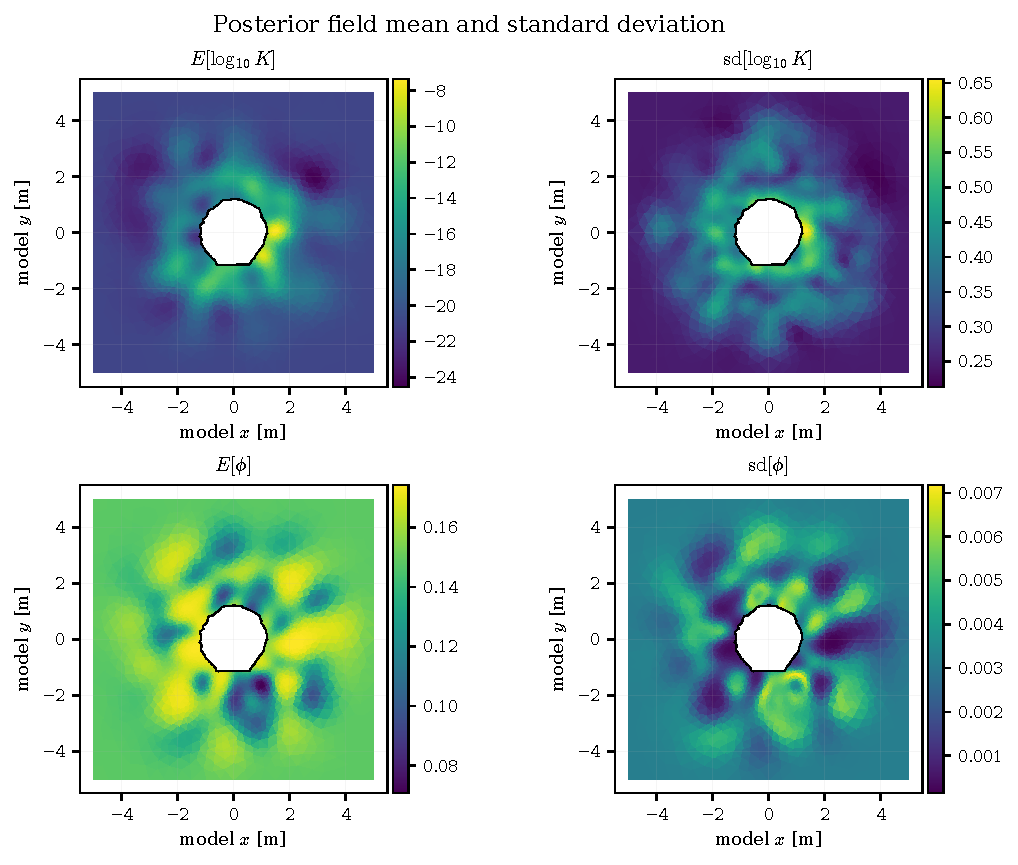
\includegraphics[width=0.98\linewidth]{fig06_posterior_field_maps.pdf}
\caption{Posterior mean and standard deviation of the permeability and porosity
fields.  The field posterior reflects the accepted trace only and should be read
as a local empirical uncertainty summary.}
\label{fig:fields}
\end{figure}

\begin{figure}[H]
\centering
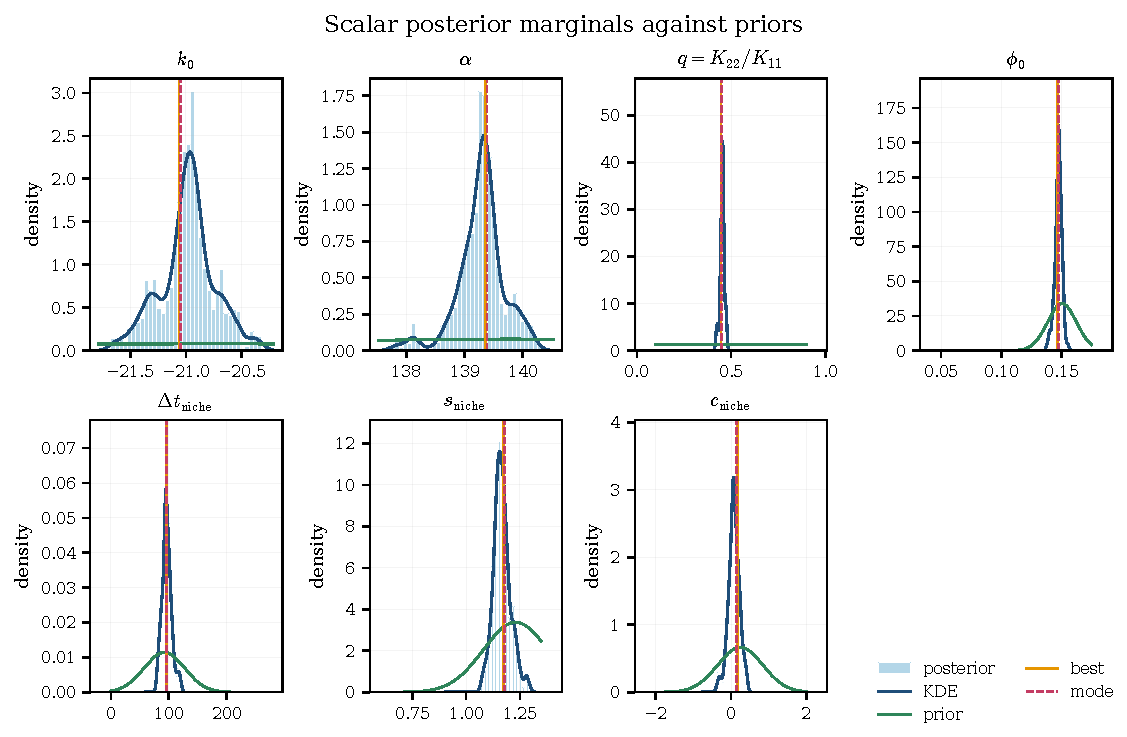
\includegraphics[width=0.98\linewidth]{fig07_scalar_posterior_priors.pdf}
\caption{Scalar posterior marginals against their configured priors.  The
posterior is much narrower than the broad configured prior for several controls,
mainly because this run started from an already-localized warm-start region.}
\label{fig:scalar-post}
\end{figure}

\begin{figure}[H]
\centering
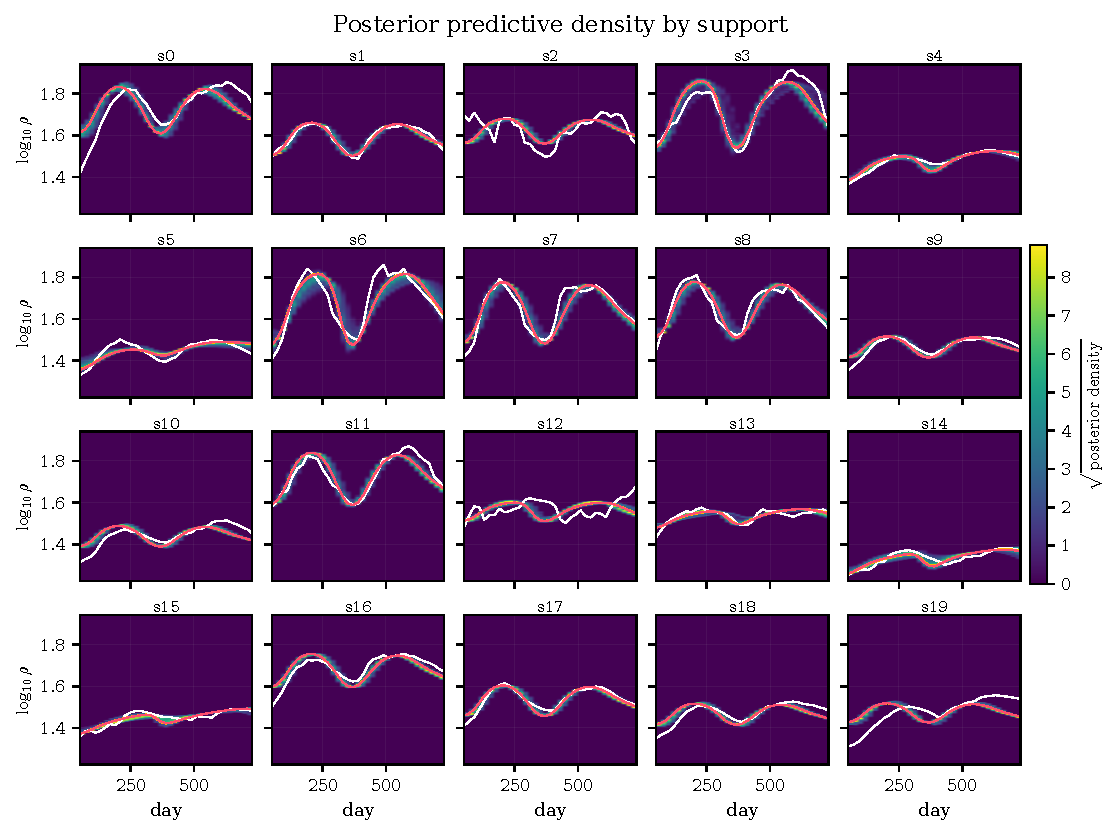
\includegraphics[width=0.98\linewidth]{fig08_posterior_predictive_pdf_20_supports.pdf}
\caption{Posterior predictive density of \(G(\thetas)\) by support.  White curves
are observations, yellow curves are the best data-fit prediction, and pink curves
are the posterior-mode prediction.}
\label{fig:pred-pdf}
\end{figure}

\begin{figure}[H]
\centering
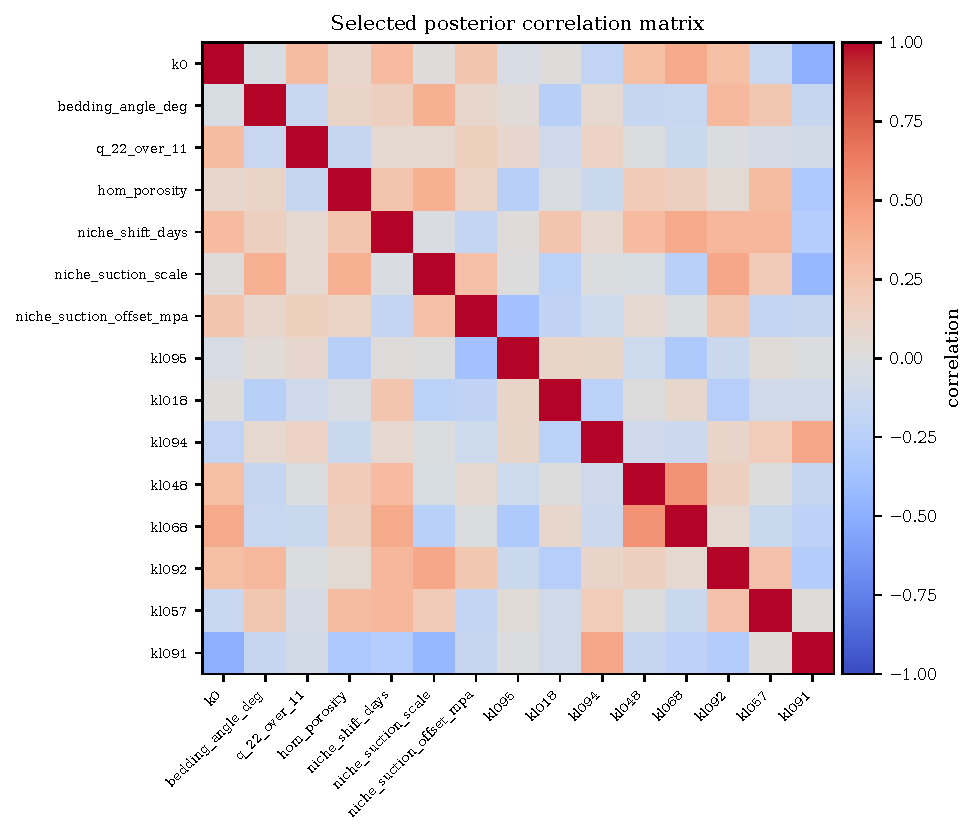
\includegraphics[width=0.82\linewidth]{fig09_selected_posterior_correlation.pdf}
\caption{Selected posterior correlation matrix for scalar controls and the KL
coefficients with the largest best-minus-prior offsets.}
\label{fig:corr}
\end{figure}

\section{Validation, Caveats, and Reuse}

The exact OGS result set is internally coherent: every indexed candidate has the
expected local files, the exact dataset has \(2083\) samples, the Archie fit table
has \(2083\times20\) rows, and residual diagnostics pass.  The surrogate validation
passed on CUDA for the warm-start and combined-live checkpoints, with
\(207\) input features and \(700\) outputs.  The missing combined-final checkpoint
is allowed by the validation summary because final retraining did not run after
the strict closeout failed.

\begin{table}[H]
\centering
\small
\begin{tabular}{p{0.24\linewidth}p{0.18\linewidth}p{0.48\linewidth}}
\toprule
Gate & State & Evidence \\
\midrule
Residual diagnostics & passed & 0.041906 RMSE; 0 issues \\
Rank diagnostics & complete & 16 MPI ranks, 15 exact solver ranks \\
Checkpoint validation & passed & 2 evaluated of 3 checkpoints; device cuda \\
Campaign status currentness & ready & 0 incomplete candidate dirs \\
Strict closeout & not complete & pending \\
Timing audit & failed & no live process; clean finish marker absent \\
Final combined MLP & dry\_run & not trained automatically after MPI shutdown caveat \\
\bottomrule
\end{tabular}

\caption{Completion and validation evidence.  The table deliberately separates
scientific artifact validity from the failed strict finish-marker gate.}
\label{tab:caveats}
\end{table}

\section{Conclusion}

The DAMH--SMU ERT20 inversion produced a dense, internally consistent exact OGS
candidate ensemble in a localized region of the CD-A Niche 4 parameter space.  The
best candidates fit the 20 support time series to about \(0.0284\) log10 MAE after
per-support local Archie calibration.  The inferred scalar controls cluster around
\(k_0\approx -21.0\), \(\phi_0\approx0.147\), \(q\approx0.45\), and an open-niche
curve shift of roughly \(96\) days.  Field posterior maps show where permeability
and porosity remain uncertain under this localized posterior, while the posterior
predictive density confirms that most observations lie close to the high-density
predictive band.

For subsequent use, the safest interpretation is: use the exact candidate set,
posterior diagnostic tables, and best-fit artifacts; label the posterior as
empirical/local rather than converged; and do not claim the final combined MLP
checkpoint exists unless a separate manual retraining run is performed and audited.

\appendix
\section{Artifact Pointers}

\begin{itemize}
\item Campaign directory: \path{/home/beremi/repos/gesa_mails/inversion_atempt/results/damh_ert20_surrogate/damh_ert20_smu_until_20260612_0830_v1}
\item Exact dataset: \code{exact_training_dataset.npz}
\item Combined dataset: \code{combined_training_dataset.npz}
\item Trace: \code{surrdamh_parameter_trace.npz} and \code{surrdamh_parameter_trace.csv}
\item Posterior summary: \code{DAMH_ERT20_POSTERIOR_summary.json}
\item Main generated report source: \code{DAMH_ERT20_RESULTS_REPORT.md}
\item This paper builder: \code{damh_ert20_inversion_paper/scripts/build_paper.py}
\end{itemize}

\end{document}
